\documentclass[10pt]{article}
\usepackage[polish]{babel}
\usepackage[utf8]{inputenc}
\usepackage[T1]{fontenc}
\usepackage{amsmath}
\usepackage{amsfonts}
\usepackage{amssymb}
\usepackage[version=4]{mhchem}
\usepackage{stmaryrd}
\usepackage{graphicx}
\usepackage[export]{adjustbox}
\graphicspath{ {./images/} }

\title{Zadania - etap I (gimnazjum) }

\author{Oświadczenie\\
Niniejszym oświadczam, że jako uczestnik konkursu „OD SZKOLNIAKA DO ŻAKA" zorganizowanego przez Centrum Nauczania Matematyki i Kształcenia na Odległość Politechniki Gdańskiej, wyrażam zgodę na przetwarzanie moich danych osobowych w zakresie niezbędnym dla potrzeb niniejszego konkursu.\\
Przyjmuję do wiadomości, że moje dane osobowe będą wykorzystane zgodnie z ustawą z dnia 29 sierpnia 1997 r. o ochronie danych osobowych (Dz.U. z 2002 r. nr 101, poz. 926 ze zm.) dla celów przeprowadzenia w/w konkursu.\\
Jednocześnie oświadczam, że zostałem poinformowany o tym, że:\\
- Administratorem danych osobowych konkursu jest: Politechnika Gdańska z siedzibą przy ul. Gabriela Narutowicza 11/12; 80-233 Gdańsk\\
- Przysługuje mi prawo do wglądu do moich danych i żądania ich poprawienia.\\
- Dane będą przetwarzane dla realizacji konkursu.\\
- Podanie danych jest dobrowolne.\\
- Nie przewiduje się przekazywania danych.}
\date{}


\begin{document}
\maketitle
CENTRUM NAUCZANIA MATEMATYKI\\
I KSZTALCENIA NA ODLEGtOŚ

Zadanie 1. Długość prostokąta powiększono o \(p \%\), a szerokość zmniejszono o \(p \%\) i otrzymano prostokąt, którego pole zmniejszyło się o \(16 \%\) względem pola pierwotnego prostokąta. Oblicz \(p\).

Zadanie 2. Długości boków pewnego trójkąta są liczbami pierwszymi. Jeden z boków ma długość 3 cm , a drugi 5 cm . Oblicz obwód tego trójkąta.

Zadanie 3. Czworokąt ABCD na poniższym rysunku jest kwadratem. Jeżeli kąt OND wynosi \(60^{\circ}\), to ile wynosi miara kąta COM?\\
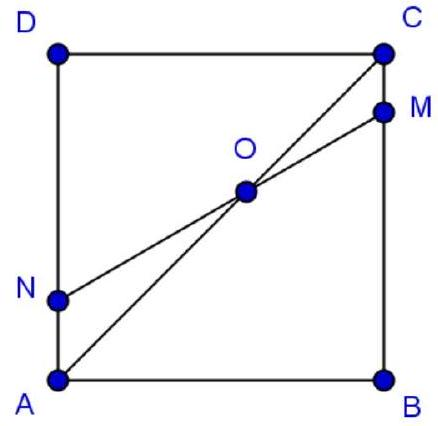
\includegraphics[max width=\textwidth, center]{2024_11_21_b612b1d0f88400ae5b9fg-1}

Zadanie 4. Pewna liczba naturalna przy dzieleniu przez 5 daje resztę 3. Jaką resztę otrzymamy dzieląc kwadrat tej liczby przez 5?

Zadanie 5. Na statku pewnego kapitana było 31marynarzy o średniej wieku 23lata. Jeżeli doliczymy wiek kapitana, to średnia wzrośnie do 24 lat. Ile lat miał kapitan?\\
\(\qquad\)

\section*{ZAŁACZNIK DO KARTY UCZESTNIKA KONKURSU „OD SZKOLNIAKA DO ŻAKA" }
Wyrażam zgodę na uczestnictwo mojego dziecka w konkursie „OD SZKOLNIAKA DO ŻAKA"

Data r.\\
(podpis rodzica lub opiekuna prawnego ucznia)

\begin{abstract}
Akceptuję i wyrażam zgodę na postanowienia regulaminu konkursu „OD SZKOLNIAKA DO ŻAKA" zamieszczonego na stronie internetowej konkursu: http:/lpg.edu.pl/kursy-z-matematyki/o-konkursie
\end{abstract}

Data r.


\end{document}